% Repository:  https://github.com/chiehrosswang/TRB_LaTeX_tex
%
% Transportation Research Board conference paper template
% version 4.0 Lite (updates made to be compatible in Overleaf and ShareLaTeX)
% 
% 
% When numbered option is activated, lines are numbered.
\documentclass[numbered]{trbunofficial}
\usepackage{graphicx}

% \usepackage[colorlinks=true,linkcolor=blue,citecolor=blue]{hyperref}
% For TRB version hide links
\usepackage[hidelinks]{hyperref}

\usepackage{orcidlink}

% Put here what will go to headers as author
\AuthorHeaders{\textit{Zinia, Bhandari, Tuffour, and Hong}}
\title{A GIS-Based Accessibility Analysis on Transit Equity in Salt Lake County}

% TODO: add macros for easier formatting of \author.
\author{%
  \textbf{Faria Afrin Zinia, Corresponding Author\,\orcidlink{0000-0001-6525-1968}}\\
  Department of City \& Metropolitan Planning\\
  University of Utah, Salt Lake City, UT 84112\\
  Email: faria.afrin.zinia@utah.edu\\
  \hfill\break% this is a way to add line numbering on empty line
  \textbf{Pukar Bhandari\,\orcidlink{0000-0002-1043-2937}}\\
  Department of City \& Metropolitan Planning\\
  University of Utah, Salt Lake City, UT 84112\\
  Email: pukar.bhandari@utah.edu\\
    \hfill\break%
  \textbf{Justice Prosper Tuffour\,\orcidlink{0000-0001-8672-6854}}\\
  Department of City \& Metropolitan Planning\\
  University of Utah, Salt Lake City, UT 84112\\
  Email: justice.tuffour@utah.edu\\
    \hfill\break%
  \textbf{Andy Hong\,\orcidlink{0000-0002-1295-1431}}\\
  Department of City \& Metropolitan Planning\\
  University of Utah, Salt Lake City, UT 84112\\
  Email: a.hong@utah.edu\\
}

% If necessary modify the number of words per table or figure default is set to
% 250 words per table
% \WordsPerTable{250}

% If words are counted manually, put that number here. This does not include
% figures and tables. This can also be used to avoid problems with texcount
% program i.e. if one does not have it installed.
% \TotalWords{200}

\begin{document}
\maketitle

\section{Abstract}

 The gap between the demand for and supply of transportation infrastructure is a major problem, which could result in the inequitable distribution of resources. In this study, we examined social equity dimensions of transportation in terms of the distribution of accessibility to light rail transit (LRT) stations in Salt Lake County, US. This research employed two novel methods seldom used in transportation research. First, we used the Two-Step Floating Catchment Area (2SFCA) method to consider both demand and supply aspects of public transit accessibility. Second, we developed spatial models to account for spatial autocorrelation issues in our data. Results showed little evidence of inequitable access to light rail transit in Salt Lake County. The accessibility to LRT stations was generally higher in the downtown and west side of Salt Lake City, where there is a concentration of low-income ethnic minority populations. We also found evidence of higher transit accessibility associated with households without a home and car ownership. Findings suggest that the light rail transit investments in Salt Lake Valley adequately addressed social equity issues.

\hfill\break%
\noindent\textit{Keywords}: Accessibility, 2SFCA, Public Transit, Light Rail, Transit Equity, Spatial Autocorrelation
\newpage

\section{Introduction}
Accessibility indicates people’s ability to connect with desired services and activities, which is the absolute goal of most transportation planning \cite{Litman2021}.  These services and activities mainly include but are not limited to education, health, housing, and employment opportunities.  Increased accessibility to such places by public transit is associated with community livability and economy, which results in the paradigm shift to accessibility-based transportation planning growth \cite{Hansen1959,Iacono2010,Litman2021}.  But the level of accessibility to these services varies spatially due to the variation in the allocation of transport resources and socio-demographic factors (like residential location, age, race, car ownership, etc.) indicating a gap between the supply and demand of public infrastructures \cite{Neutens2015}.  This two-sided phenomenon of spatial accessibility establishes the necessity of assessing both demand and supply in accessibility studies.

Having said that, the commonly used typology of accessibility studies, including frequency-based access and opportunity-based access \cite{Xavier2021}, suggests that the gravity-based model, which only considers the supply side leaves room for further research considering its demand side.  In other studies utilizing cumulative opportunities accessibility, the demand side has been considered \cite{Ermagun2020,NazariAdli2019}. However, one of the efficient and advanced method; two step floating catchment area (2SFCA) analysis which considers both of demand-supply side enabling the shortage calculation of public transit has not been used. 2SFCA is one of the vital and most commonly used methods of accessing spatial accessibility due to its easy and advanced application \cite{Tao2020}. Although it’s widely used in geography, especially in measuring spatial accessibility to healthcare, this approach is completely novel in transit equity analysis as per author’s best knowledge, indicating the need for research to utilize this method.
 
However, after resolving the accessibility measurement method, the next question comes how are the facilities distributed? If they are equitably distributed regardless of socio-economic condition, race, and so on? To address these questions, several prominent researchers have assessed the equity of transit accessibility \cite{Ermagun2020,Jang2017,Karner2018,NazariAdli2019,Xavier2021}.  As transit accessibility to essential services and activities is required irrespective of any class and race in the society to make the economy thrive, and the inaccessibility of these large groups to opportunities can lead to social exclusion, resulting in increased social and transportation inequities, equity research deals with the distribution of transportation burden and benefits \cite{Bierbaum2021,Karner2018,Lucas2012}.  Usually, these studies analyze the distribution of accessibility by different socio-demographic cohorts using Gini Coefficient, Descriptive Statistics, and Regression Models \cite{NazariAdli2019,Xavier2021}.

To integrate two fundamental aspects of transportation planning which are equity and transit accessibility, and understanding the need to advance the accessibility study, in this research, we are adopting the widely used geographical spatial accessibility technique 2SFCA into transit station accessibility analysis to enlarge the methodological approach of accessibility study and assessing the equity using regression models.  We are materializing our research idea within Salt Lake County; with taking account of only light rail services as finding of Victoria Transport Policy Institute’s research from 130 cities suggests that light rail services are associated with high accessibility the motivation of the negative transport externalities like traffic congestion, inefficient land use disposition, housing affordability, air pollution \cite{Litman2012}.  In addition to that, in 2018, the average capital cost for an existing light rail system was much higher than the bus rapid services, where right rail cost \$30.6 million, and bus cost 1.1 million with a 225\% more vehicle maintenance cost and 346 percent facility maintenance cost than bus rapid services \cite{FederalTransitAdministration2019}.  This substantial light rail investment consisting of a large share of taxpayers’ money requires the equitable distribution of its benefits and burden, which is the economic rationale of working with light rail in this research.

The subsequent section of this research is organized as follows.  First, we reviewed the existing literature on transit equity and accessibility measurement methods.  Second, we briefly illustrate the study area context. Third, we described the data and methods we used to conduct this study.  Fourth, we provided an in-depth discussion on our result and analysis.  Finally, we wrap off the study with a summary of the important findings, planning recommendations, and future research directions.

\section{Literature Review}

\subsection{Transit Accessibility}
For most of transportation planning history, the efficiency of the transportation system has been measured in terms of ‘mobility’ or ‘level of service’, which measures the ease of movement from origin to destination. While mobility focuses on movement, it barely connects the movement to the landuse compatibility and the opportunities of destinations to the city residents. This focus on mobility has, over the decades, resulted only in wider roads, increasing vehicular speeds, and the resulting harm it has caused; such as unsustainable urban sprawl, traffic crashes, etc. Therefore, as early as 1959, there had been efforts of introducing and defining the early measures of accessibility. \citep{Hansen1959} defines accessibility as “.. a measurement of the spatial distribution of activities about a point, adjusted for the ability and the desire of people or firms to overcome spatial separation.” In general, accessibility can be understood as the ease of reaching the desired destination from a specified location \cite{NazariAdli2019}, a characteristic advantage of a said location in terms of the number of available opportunities with respect to overcoming some spatial friction or impedance \cite{Ingram1971}. Commonly, the desired destinations are tied to the economic opportunities whereas the impedance is measured in terms of distance or travel time to the destination from the origin.

Although we have established a general definition of accessibility, however, the standard definition of accessibility measures has not been established yet. As a result, there have been a number of efforts by various authors and researchers to develop a model or measure to assign a numeric value to the accessibility of a place. Most of these researches boil down to the following categories of accessibility measures: (i) Infrastructure-based Models, (ii) Graph Theory and Spatial Separation (Distance) Measures, (iii) Cumulative Opportunities Models, (iv) Gravity Measure, (v) Utility Measure, and (vi) Time-Space Measure \cite{Geurs2001,Bhat2000,Pirie1979,Koenig1980}. Development of these accessibility measures have been primarily intended to understand the characteristic feature of a given location based on transportation options, landuse distribution, time, and individual choices. These are also called the components of accessibility \cite{Geurs2001}. These features help us understand and describe the effects of landuse and transportation on each other, analyze the impacts of proposed transportation projects, find suitable landuse interventions, and even highlight the differences in impacts between various population groups \cite{Bhat2000,Pirie1979}. These quantification measures of accessibility would enable us to reflect upon the interaction of people with the built environment, which in turn would help analyze the social inequities within our cities \cite{Bhat2000}.

As cities are ever-expanding, the resulting issues such as congestion, sprawl, and sustainability make it obvious that public transit is the optimal mode of transportation. Multiple studies have shown that strengthening public transit would contribute to increased accessibility to opportunities throughout the demographics \cite{Stern2020}. Transit accessibility is also important because it is one mode of transportation that can bridge existing socio-economic inequalities by providing a quality mode of transportation to various social and economic opportunities. There are two basic analyses of transit accessibility, namely: accessibility to transit and accessibility by transit. Accessibility to transit has been considered as a measure to analyze the access to public transit services from the places of residence, primarily focused on access to public transit options and stops. While on the other hand, accessibility by transit discusses the access to opportunities spread out throughout the city, through network connectivity of transportation options. These two transit accessibility analyses should be studied individually to avoid misleading inferences and erroneous policy prescriptions \cite{Moniruzzaman2012}. In this research, we are primarily focused on accessibility to public transit and the availability of public transit at various block group levels within Salt Lake County. This would help us analyze if the public transit access has been serving the various distribution of demographic groups throughout the metropolitan region.

\subsection{Social Equity}
The definition and classification of equity in recent studied have been adapted from Litman, 2005  where categorize the equity into horizontal equity and vertical equity \cite{Delbosc2011,Foth2013,Xavier2021}. In horizontal equity, each individual and group are treated equally in resource and cost distribution. As horizontal transit equity ensures the uniform spatial distribution of transit facilities, it disregards the population densities and regional/urban characteristics to access the need for public transit \cite{Foth2013}. On the contrary, vertical transit equity, also referred to as transit justice, advocates for the distribution of transit resources among individuals or groups with different abilities and needs, thus favoring groups depending on social class or specific requirements to offset societal disparities \cite{Delbosc2011}.

As transit accessibility has a direct impact on disadvantaged groups’ livelihood, which can result in social exclusion \cite{DiCiommo2017}, in this research, we aim to access the vertical equity in the distribution of Utah light rail stations throughout the Salt Lake County using spatial autoregressive models.

Limited research has been conducted on transit equity for Utah and Salt Lake City. The white paper attempted to discuss transit equity in terms of home-to-workplace accessibility during the pandemic, but accessibility to the public station was not covered \cite{Loayza2022}. Although Salt Lake City partnered with the Utah Department of Transportation (UDOT), Utah Transit Authority (UTA), and Wasatch Front Regional Council (WFRC), to assess the walking accessibility to the transit stop, it was at the neighborhood scale of Westside of Salt Lake City \cite{SLC2021}. Thus, observing the need for a walking accessibility analysis for Salt Lake County, this research considers the whole of Salt Lake County as the study area.

\section{Data and Methods}

\subsection{Study Context}
With a view to increase accessibility through public transit and bolster a polycentric development pattern in the Salt Lake metropolitan region, Utah Transit Authority (UTA) introduced light rail services branded as UTA TRAX to enhance transit ridership and connectivity to shared community destinations throughout the Salt Lake valley \cite{UtahTransitAuthority2022}.

In spite of these vigorous transit-focused agenda and plan implementation (provision of UTA TRAX and UTA bus services), there appear to be public interest questions on the resultant impacts. Currently, 12\% of renter households and 2\% of owner-occupied households in Salt Lake County have no car, thus solely dependent on public transit \cite{U.S.CensusBureau2019}.  The race-wise distribution of car ownership further demonstrates that 15\% of black, 8\% of Asian or Pacific Islanders, and 5\% of White/Latino households depend on public transit to access jobs and basic amenities as they do not have any car (\cite{PolicyLink2019}. So, the question remains if the public transit of Salt Lake County is effectively supporting the mobility demand of these large groups or if they are discriminatory in the provision of access to such opportunities. Moreover, the Civil Rights Act of 1964 Title VI prohibits federally funded transit providers such as the UTA from administering programs "…. in ways that would subject individuals to discrimination based on their race, color or national origin" \cite{Farber2014}; there exist some concerns of inadequate accessibility and displacement-related issues particularly affecting the racial and socio-economic minority communities.

Although it is believed that the transit system has expansively connected the public to essential services and opportunities like shopping centers, schools and universities, Frontrunner stations, bus hubs, and Park \& Ride lots, this research will answer the following questions question of its equity it's station's accessibility.

\begin{figure}[!ht]
  \centering
  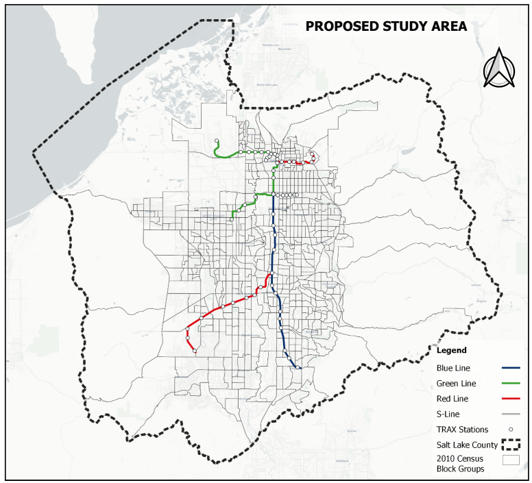
\includegraphics[width=0.8\textwidth]{Study Area.png}
  \caption{Study Area}\label{fig:trial}
\end{figure}

\subsection{Indicators of Social Equity}
While the concept of social equity has been around for years, only a handful of research provides a framework to empirically measure and understand their performance to achieve equity outcomes \cite{Appleyard2019}. Owing to the fact that equity can be examined from a variety of perspectives, the study specifies the social equity indicators used for the analysis and the sources they are derived from for replicability purposes. For instance, in previous studies like \citep{Dill2009}, racial and ethnic minorities, families living below the poverty line, children under the age of 18, seniors over the age of 65, and people who speak little English have all been considered historically underserved populations in their analysis. Surmising such previous research on the subject matter, this study adopts eight (8) commonly used social equity indicators. These indicators are household income, race, ethnicity, age, employment, education, vehicle ownership, and house ownership. Adapted from the existing pieces of literature, the equity variables we used in this study, along with their descriptive statistics, are as follows:

\begin{table}[!ht]
	\caption{Summary of Variables by Blockgroups}\label{tab:versions}
        \begin{small}
	\begin{center}
		\begin{tabular}{p{0.5in}|p{1.1in}|p{0.2in}|p{0.3in}|p{0.3in}|p{0.3in}|p{0.3in}|p{0.3in}|p{0.3in}|p{0.4in}|p{0.3in}|p{0.2in}}
            \hline
            \textbf{Variable} & \textbf{Description} & \textbf{Min} & \textbf{Q1} & \textbf{Median} & \textbf{Mean} & \textbf{Q3} & \textbf{Max} & \textbf{SD} & \textbf{Variance} & \textbf{IQR} & \textbf{NA's} \\\hline
                Age & Percentage of dependent groups (i.e., less than 18 and over 65 years) & 3.981 & 32.506 & 38.347 & 37.107 & 43.092 & 61.345 & 8.939 & 79.914 & 10.586 & 1\\
                Household Income & Percentage of households with income less than 80 percent of the Area Median Income (74,865 USD) & 0.000 & 23.700 & 37.559 & 39.410 & 53.880 & 89.024 & 19.052 & 362.977 & 30.175 & 2\\
                Race & Percentage of non-White population & 0.000 & 7.343 & 14.828 & 20.130 & 30.268 & 86.616 & 16.640 & 276.876 & 22.925 & 1\\
                Ethnicity & Percentage of the Hispanic population & 0.000 & 4.608 & 11.876 & 17.835 & 26.949 & 81.726 & 16.789 & 281.875 & 22.340 & 1\\
                Employment & Percentage of the unemployed civil population & 0.000 & 1.335 & 2.895 & 3.660 & 4.975 & 21.165 & 3.357 & 11.270 & 3.640 & 2\\
                Education & Percentage of population over 25 years with less than a High School Diploma & 0.000 & 1.534 & 4.208 & 6.009 & 9.213 & 38.211 & 5.866 & 34.410 & 7.679 & 1\\
                Vehicle Ownership & Percentage of Households who do not own Vehicles & 0.000 & 0.000 & 2.510 & 4.885 & 6.625 & 50.224 & 6.937 & 48.127 & 6.625 & 2\\
                Home Ownership & Percentage of Renter-occupied Households & 0.000 & 10.320 & 24.485 & 31.187 & 47.820 & 100.000 & 25.393 & 644.816 & 37.500 & 2
                \\\hline
		\end{tabular}
	\end{center}      
        \end{small}
\end{table}

Given the contextual scope of the study (i.e., Salt Lake County) and the nature of the variables needed to analyze the research, elaborate sampling and first-hand data collection strategies were not requisite. We, therefore, obtained data from secondary sources (i.e., publicly available data sources) that were relevant to the unit of analysis. The demographic dataset of the socio-economic indicators have been adopted from the 2019 5-year American Community Survey at the block-group level, whereas the geospatial dataset of the UTA-TRAX services, route, and stops have been obtained from \href{https://gis.utah.gov/data/transportation/transit/#UTALightRailStations}{Utah Geospatial Research Center}. The isochron buffers of the service area around the TRAX stations were created using the \href{https://github.com/GIScience/openrouteservice-r}{OpenRouteServices} API key.

In terms of data analysis tools, we adopt Data Analytics and GIS-Based software like R programming, \href{https://github.com/tidyverse}{Tidyverse}, \href{https://github.com/walkerke/tidycensus}{Tidycensus}, and QGIS to examine the nature of social equity within a 15-minute walking radius of transit station areas. Concerning the advanced GIS techniques, the study uses spatial accessibility mapping procedures, spatial filtering and joining of census data with Salt Lake County geospatial data, and a 2 Step Floating Catchment Area analysis (2SFCA). The 2SFCA method to be employed is an analytical method for combining several related types of information (i.e., indicators for social equity) into a meaningful index that allows comparisons to be made across different locations (i.e., transit station areas). Moreover, spatial accessibility mapping is a spatial analytical technique that evaluates the physical range and minimum distance for a specific group of people to access a facility or infrastructure.

\subsection{Two-Step Floating Catchment Area Analysis}
The two-step floating catchment area (mostly called 2SFCA) is an extensively adapted quantitative method that allows for comparative analysis across different locations using a justifiably derived index. Over the decades, the 2SFCA has increasingly emerged as a key measure for spatial accessibility research, with current enhancements leveraging the shortfall of distance decay \cite{KC2020,Langford2016,McGrail2012,Luo2009}. For instance, recent applications of 2SFCA have measured the differentials in spatial accessibility at the micro-scale to reflect the balance between supply and demand of public facilities like healthcare and education \cite{Li2022,Wu2020}. This paper entails three main steps detailing the culmination of a 2-Step Floating Catchment Area and multiple regression analysis. The first step comprises extracting census block group and TRAX station data for spatial joins. We calculate the supply ratio of TRAX stations for each station area by deriving the transit frequency and ridership capacity. The transit frequency is computed by summing the number of TRAX lines that run through each transit station and the number of times each line stops at that station each day. Again, the ridership capacity is derived by multiplying the seating supply by the average number of railcars (i.e., 3). Step two continues by defining a 20-minute walking radius or buffer around every transit station area at the census block group level and joining the resultant catchment area with the already computed supply ratio. A supply-demand ratio is computed by finding the population to transit supply per capita for each transit station area – to derive a spatial accessibility value.

\subsection{Spatial Autocorrelation \& Multiple Regression Analysis}
Spatial autocorrelation is a statistical model that demonstrates the clustering or dispersion in a systematic spatial variation of observed variables (i.e., spatial dependence) – mostly measured by the Moran’s I index. As a rule of thumb, the presence of autocorrelation in an observation violates the statistical assumption of independence within and between groups of observations \cite{Freitas2022,Mahrous2022,Fischer2011}. Technically, the presence of spatial autocorrelation can be expressed by:

\begin{linenomath}
  \begin{equation}
    Cov(y_i,y_j) = E(y_i,y_j) - E(y_i)E(y_j),i \neq j
  \end{equation}
\end{linenomath}

Where $(y_i)$ and $(y_j)$ are observations on a random variable at locations $(i)$ and $(j)$ in space, and $(i)$, $(j)$ can be points (i.e., measured as latitude and longitude or areal units). In this regard, the value of a variable of interest in each region $(i)$ is associated with the value of the same variable in the neighboring regions $(j)$. Similar to other studies, the empirical application of spatial autocorrelation in this paper is to measure social equity or disparities in accessibility to selected transit stations using the Moran’s I coefficient \cite{Li2020,Zhu2018}. The third step is a quantitative analysis of assessing the impact of the spatial accessibility of TRAX on the specified social equity indicators using standard linear regression models. The process is finalized by empirically selecting the best spatial model to interpret the resultant impact of transit accessibility on the social equity indicators.

\section{Findings}

\subsection{Accessibility to Transit}
The 2SFCA analysis of accessibility of census block groups to the UTA TRAX stations shows that the accessibility to the TRAX stations in Salt Lake County is generally higher in the block groups that are within walking distance from the stations. Particularly, the block groups within and near the downtown and in the center of Salt Lake City, around the center of West Valley City, and near the Murray-Draper have much higher accessibility than the other block groups adjacent to the TRAX lines. This finding is a reflection of these block groups having high population density as well as multiple stations within relative proximity of each other, thus effectively increasing the accessibility to the TRAX station for a higher population than the rest of the county. These areas have a high population density as well as multiple stations within relative proximity of each other, thus effectively increasing the accessibility to the TRAX station for a higher population than the surrounding area.

\begin{figure}[!ht]
  \centering
  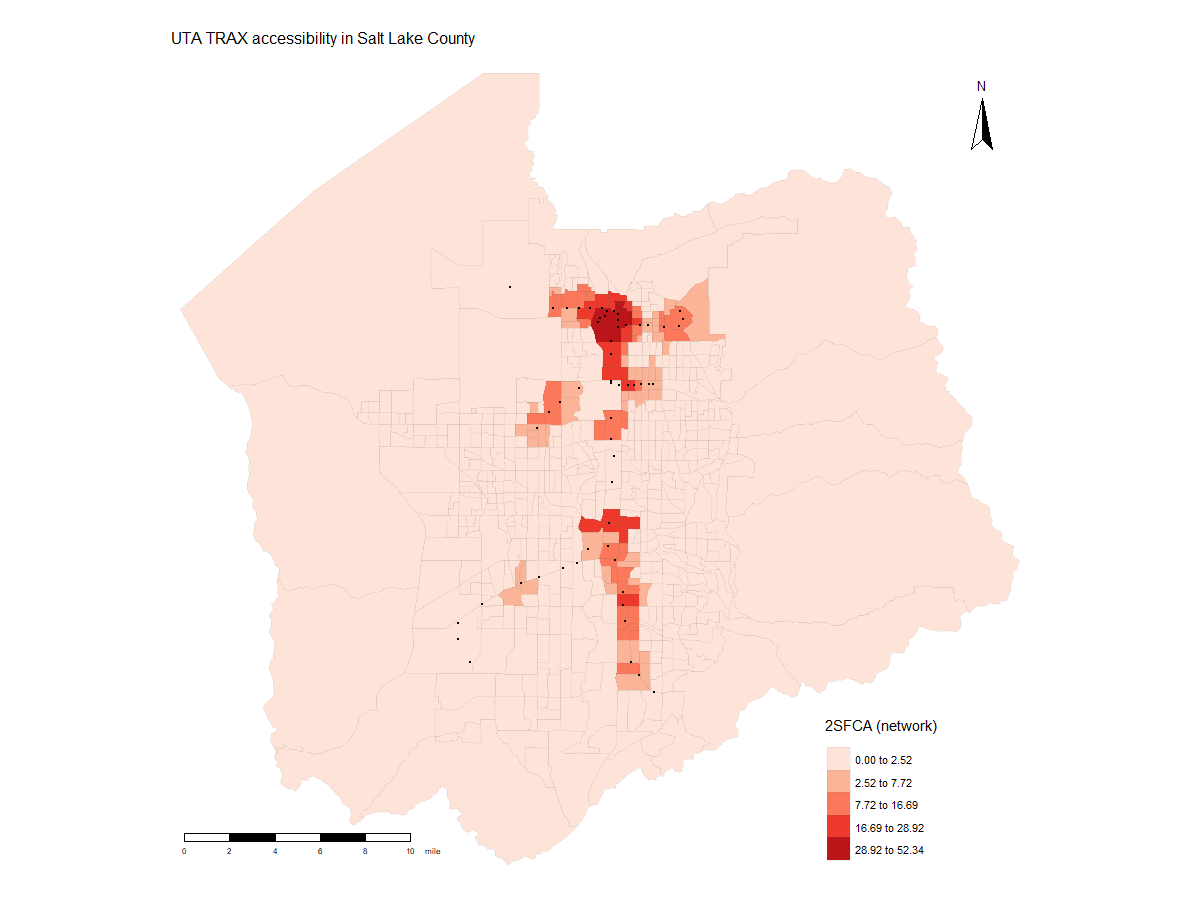
\includegraphics[width=0.8\textwidth]{TSFCA.jpg}
  \caption{UTA TRAX Accessibility in Salt Lake County}\label{fig:trial}
\end{figure}

\subsection{Ordinary Least Square Regression Model}

In order to quantify the relationship between social equity variables and transit (UTA TRAX) accessibility, the Ordinary Least Square method was adopted. This model suggested that the population within the dependent age group (below 15 and above 65), percentage of renter households, and percentage of households with no car significantly impact transit accessibility. However, the model had a very low R2 value. Upon further analysis, the residual histogram and the Q-Q plot of the data pattern demonstrated that the data are not normally distributed and violate the assumption of the Independent and Identically distributed (IID) random variables property. The Moran's I test further illustrated a spatial correlation using the Queen's Contiguity matrix. The Lagrange Multiplier (LM) diagnostic test, a widely used test to check for spatial dependence, also demonstrated significant LM and Robust LM (RLM) statistics for both the spatial error and spatial lag models, indicating the need to implement spatial auto-regressive models for further analysis.

\subsection{Spatial Auto-regressive Models}
Taking the spatial autocorrelation into consideration, two autoregressive models; Spatial Lag Model and Spatial Error Model have been developed. The spatial lag model addresses spatial dependency in a spatial unit's dependent variable and its surrounding units. In contrast, the spatial error model considers geographic dependence in a spatial unit's error term and its neighboring units \cite{Saputro2019}.

The Spatial Lag Model shows that only the percentage of households with no vehicle significantly impacted transit accessibility. In contrast, Spatial Error Model ended with no significant impact of the explanatory variables on accessibility other than the intercepts. Although the performance of both models does not significantly vary, the Spatial Lag model has been selected as the best-fitted one to describe the relationship between transit accessibility and the social equity variable as it has a lower AIC value among the two models. The Akaike information criterion (AIC) is a widely adopted measure of prediction error \cite{Aho2014} and thus reflects a relative model quality for a given set of data.

\begin{table}[!ht]
	\caption{Model Comparision}\label{tab:versions}
	\begin{center}
		\begin{tabular}{l|c c|c c|c c}
                \hline
                Variable & \multicolumn{2}{c}{Ordinary Least Square} & \multicolumn{2}{c}{Spatial Lag Model} & \multicolumn{2}{c}{Spatial Error Model}\\
			    & Estimate & p-Value & Estimate & p-Value & Estimate & p-Value\\\hline
                Intercept & 3.769 & 0.005* & 0.585 & 0.457 & 3.861 & 0.025\\
                \%NonWhite & -0.028 & 0.242 & -0.009 & 0.545 & -0.015 & 0.331\\
                \%Hispanic & 0.005 & 0.857 & -0.007 & 0.671 & -0.013 & 0.371\\
                \%Unemployed & 0.122 & 0.088 & 0.069 & 0.097 & 0.044 & 0.265\\
                \%DependentPop & -0.115 & 0.000* & -0.022 & 0.217 & -0.032 & 0.107\\
                \%NoDiploma & -0.009 & 0.893 & -0.009 & 0.810 & -0.01 & 0.794\\
                \%RenterHH & 0.044 & 0.005* & 0.011 & 0.224 & 0.013 & 0.156\\
                \%<80AMHI & 0.016 & 0.454 & -0.002 & 0.876 & -0.01 & 0.459\\
                \%NoVehicles & 0.240 & 0.000* & 0.071 & 0.003* & 0.047 & 0.060\\\hline
                \multicolumn{7}{c}{Model Performance}\\\hline
                & \multicolumn{2}{c}{$Adjusted R^2: 0.2424$} & \multicolumn{2}{c}{$Rho: 0.8764$} & \multicolumn{2}{c}{$Lambda: 0.9120$}\\
                Log-likelihood & \multicolumn{2}{c}{} & \multicolumn{2}{c}{-1,641.953} & \multicolumn{2}{c}{-1,650.228}\\
                AIC & \multicolumn{2}{c}{3836.40} & \multicolumn{2}{c}{3,305.905} & \multicolumn{2}{c}{3,322.456}\\
                LM (Robust LM) Statistic & \multicolumn{2}{c}{} & \multicolumn{2}{c}{624.1029 (91.1694)} & \multicolumn{2}{c}{535.6696 (2.7361)}\\\hline
		\end{tabular}
	\end{center}
\end{table}

\subsection{Model Explanation}
The final model to define the relationship between transit accessibility and social equity variables from this study is as follows:

\begin{linenomath}
  \begin{equation}
    Transit Accessibility = 0.585 + 0.071 * \textit{Percent of Households who do not own Vehicles}
      \end{equation}
\end{linenomath}

According to this Spatial Lag Model, the percentage of households having no car is the only variable that has a significant impact on transit (UTA Trax) accessibility. Although the percentage of households having no vehicle, dependent population ratio, and renter household were statistically significant in the Ordinary Least Square Regression model, the latter two variables were not statistically significant (p-value greater than 0.05) when spatial autocorrelation was considered.

\section{Discussion}

The study finds that transit accessibility is generally higher for areas around 20 minutes walking distance along TRAX lines. This is reasonable, as transit accessibility scores for transit station areas are relatively higher for households within these areas. Having said that, instances of spatial clustering of accessibility has been observed in the areas around Salt Lake City Downtown, towards the University of Utah, and southbound towards Murray and Sandy. Therefore, transit agencies, MPOs, and local land-use decisions need further coordination and integration to make substantial improvements toward overcoming imbalances in transit access while optimizing the network coverage within the Salt Lake Valley. The advancement of social equity within local transit station areas relies on the efficient interplay of land use and public transit systems to leverage public benefits for social minorities.

As our study controls for about a mile radius around transit station areas, we find that there were statistically insignificant relationships between transit accessibility and social minorities living in these areas. In other words, it means that transit accessibility in Salt Lake County is inclusive of social minorities like; households categorized under dependent population, renters, non-White population, low education background, incomes below AMHI, and non-vehicle owners. Our final model (Spatial Lag Model) indicated a significant correlation between accessibility with only one of the equity variables; the percentage of households having no car, which has a significant positive impact on accessibility. Quantitatively, it means that doubling the percentage of households with no income will result in an increase in accessibility by 7.1\%. Furthermore, the other equity variables; the percent of the unemployed population and renter households within the census block group, are positively correlated with access to transit, although their impact is not significant. Therefore, the overall model indicates that an increase in accessibility to transit will favor the disadvantaged group by increasing ridership from the household with no cars, thus reducing VMT and possibly reducing vehicular ownership in the service area around the station. Furthermore, this study also finds that there is not sufficient evidence to demonstrate that the other socio-economic indicators (such as race, ethnicity, income, age, education, employment, and homeownership) have a significant impact on accessibility to transit within the study area. These findings can be explained by the population distribution within Salt Lake County in terms of race, ethnicity, and socio-economic status \cite{UtahTransitAuthority2021}. In this regard, the UTA-TRAX, in contrast to other counterarguments \cite{McKane2020,Padeiro2019,Ewing2017}, provides somewhat robust and equitably inclusive opportunities for social minorities to improve their quality of life.

In comparison to a similar transit accessibility study conducted in the cities of Chicago, Auckland, Brisbane, Perth, and Vancouver, which have found a varying degree of transportation justice and equity, our study finds that the light rail service within Salt Lake County is equitable to the social minority group. The public transit system in Chicago, Brisbane, Perth, and Auckland was found to provide relatively lower accessibility in the areas that have a higher percentage of the socio-economically disadvantaged population \cite{Ermagun2020,NazariAdli2019}, benefitting the population who live in proximity of the economic centers. Vancouver public transit services, however, have shown to provide better services for low-income families \cite{NazariAdli2019}. The studies have shown that these findings correlate to the population distribution across those cities, as the transit lines majorly serve more affluent neighborhoods within those cities. Meanwhile, our analysis found higher accessibility around the highly urbanized areas within Salt Lake County with a higher concentration of social minority groups, indicating the equity and justice in the location and routing of the light rail lines within Salt Lake County. Such equitable distribution of public transit supporting the minorities and the low-income group is the outcome of the implementation of transportation policies aiming to enhance the public transit ridership by improving access to opportunities through coordination and partnership of Salt Lake County, Wasatch Front Regional Council (WFRC), Utah Department of Transportation (UDOT), and Utah Transit Authority (UTA) \cite{WasatchFrontRegionalCouncil}.


\section{Acknowledgements}

This paper and the research behind this would not have been possible without the generous guidance and feedback from Dr. Andy Hong, Assistant Professor at the Department of City \& Metropolitan Planning, University of Utah. We are thankful for all the comments and suggestions from our fellow classmates in the CMP6455 Advanced GIS Applications course. We are very much indebted to all the people who have worked hard to create the online database of demographic data at the US Census Bureau and spatial data at the Utah Geospatial Resource Center. This acknowledgment would be incomplete without thanking the great people who have developed the R programming language, as well as the $tidyverse$, $tidycensus$, and $openrouteservices$ packages for R. We are equally thankful for all the other people who have directly or indirectly supported us during this research project.

\section{Author Contributions}

 Faria Afrin Zinia: Conceptualization, Study Design, Formal Analysis and interpretation of results. Writing-original draft manuscript preparation, validation. Justice Prosper Tuffour: Data Preparation, Data interpretation, and Original Draft Manuscript Preparation. Pukar Bhandari: Conceptualization, Study Design, Formal Analysis, and interpretation of results. Writing-original draft manuscript preparation, validation. Andy Hong:  Validation, Review, and Supervision.

\newpage

\bibliographystyle{trb}
\bibliography{trb_template}
\end{document}
